\documentclass{beamer}

\usetheme{Warsaw}
\usefonttheme{professionalfonts}
%\logo{\includegraphics[height=1cm]{./images/logo.png}}
\beamertemplatenavigationsymbolsempty
\setbeamertemplate{caption}{\raggedright\insertcaption\par}
\usepackage{amsmath}
\usepackage{amssymb}
\usepackage[spanish]{babel}
\usepackage{changepage}
\usepackage{fancyvrb}
\usepackage{float}
\usepackage{framed}
\usepackage[T1]{fontenc}
\usepackage{geometry}
\usepackage{graphicx}
\usepackage{hyperref}
\usepackage[utf8]{inputenc}
\usepackage{minted}
\usepackage{multicol}
\usepackage{relsize}
\usepackage{subcaption}
\usepackage{textcomp}
\usepackage{tikz}
\usepackage{upgreek}
\usepackage{verbatim}
\usepackage{wasysym}
\usepackage{xcolor}
\definecolor{LightGray}{gray}{0.9}

%\setbeamertemplate{footline}[frame number]

\begin{document}

\title[Lógica proposicional]{Teoría de la Computación \\ Unidad 1: Lógica
  proposicional (parte 1)} \author[Teoría de la
Computación]{cristobal.loyola@usach.cl} \date{}

\titlegraphic{
  \vspace{-1.5cm}
  \begin{figure}
    \centering
    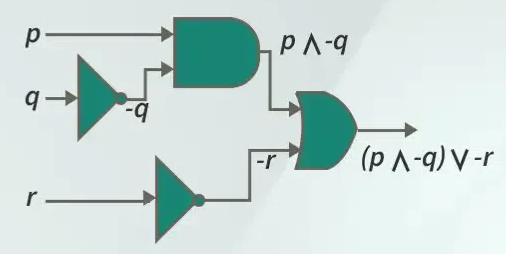
\includegraphics[width=.75\linewidth]{images/circuito_logico.png}
  \end{figure}
}

\frame{\titlepage}

\setbeamertemplate{footline}[frame number]

\begin{frame}{Contenidos}
  \begin{itemize}
    \item Formas de razonamiento y tipos de lógica.
    \item Lógica proposicional (repaso).
    \item Deducción natural.
  \end{itemize}
\end{frame}


\begin{frame}[plain,c]
  % \frametitle{A first slide}
  \vspace{1cm}
  \begin{center}
    \Huge Motivación
  \end{center}
\end{frame}


\begin{frame}{Motivación}
  Considere el problema cotidiano de decidir si llevar paraguas o no al salir de
  casa. Podemos razonar de la siguiente manera:

  \begin{itemize}[<+->]
    \item \textbf{Premisas:}
          \begin{enumerate}[<+->]
            \item Si el cielo está nublado, entonces lloverá.
            \item Si llueve y no llevo paraguas, entonces me mojaré.
            \item Hoy está nublado.
            \item No quiero mojarme
          \end{enumerate}

          \item \textbf{Conclusión:}
          \begin{itemize}
            \item Llevaré un paraguas.
          \end{itemize}
  \end{itemize}

  \begin{figure}
    \centering
    
\includegraphics[width=.55\linewidth]{images/paraguas.png}
  \end{figure}
\end{frame}


\begin{frame}{Motivación}
  Algunas formas de razonamiento son:
  \begin{itemize}[<+->]
    \item \textbf{Razonamiento deductivo:} parte de premisas generales para
          llegar a una conclusión necesariamente verdadera (si las premisas son
          verdaderas).

          \begin{itemize}
            \item \textbf{Ej:} Todos los humanos son mortales. Alan Turing es
                  humano. Por lo tanto, Alan Turing es mortal.
          \end{itemize}
    \item \textbf{Razonamiento inductivo:} usa premisas específicas para llegar
          a una conclusión probable (no segura).
          \begin{itemize}
            \item \textbf{Ej:} El sol ha salido todas las mañanas hasta hoy. Por
                  lo tanto, mañana saldrá el sol (es probable, pero no está
                  garantizado).
          \end{itemize}
  \end{itemize}
\end{frame}


\begin{frame}{Motivación}
  Algunos tipos de lógica son:
  \begin{itemize}[<+->]
    \item \textbf{Lógica proposicional:} estudia proposiciones simples
          (verdaderas o falsas) y su combinación mediante conectores.
    \item \textbf{Lógica de primer orden:} incluye predicados, cuantificadores y
          variables.
    \item \textbf{Lógica difusa:} trabaja con grados de verdad (no sólo
          verdadero / falso).
  \end{itemize}
\end{frame}


\begin{frame}{Motivación}
  ¿Qué es y cómo se caracteriza una lógica?
  \begin{itemize}
    \item \textbf{Sintaxis:} define las reglas para construir expresiones
          válidas (fórmulas bien formadas).
    \item \textbf{Semántica:} asigna un significado a las expresiones (valores
          de verdad, interpretaciones).
    \item \textbf{Sistema de inferencia:} establece reglas para derivar
          conclusiones a partir de premisas.
    \item \textbf{Consistencia:} no debe admitir contradicciones\footnote{No
          obstante, existen lógicas paraconsistentes.}.
    \item \textbf{Completitud:} toda fórmula válida puede ser demostrada a
          partir de las reglas del sistema\footnote{La lógica de primer orden es
          completa, pero no decidible: no existe un algoritmo general que
          determine si una fórmula cualquiera es válida.}.
  \end{itemize}
\end{frame}


\begin{frame}[plain,c]
  % \frametitle{A first slide}
  \vspace{1cm}
  \begin{center}
    \Huge Lógica proposicional
  \end{center}
\end{frame}


\begin{frame}{Lógica proposicional}
  Una \textbf{proposición} es un enunciado declarativo que puede ser verdadero o
  falso, pero no ambos a la vez.

  ¿Cuáles de los siguientes enunciados son proposiciones?

  \begin{enumerate}[<+->]
    \item El sol es una estrella.
    \item 8 es un número impar.
    \item ¿Qué hora es?
    \item La pizarra es negra.
    \item Por favor, cierra la ventana.
    \item Este enunciado es falso.
    \item No está soleado afuera.
  \end{enumerate}
\end{frame}


\begin{frame}{Lógica proposicional}
  Las proposiciones pueden ser:
  \begin{itemize}[<+->]
    \item \textbf{Atómicas:} no se pueden descomponer en proposiciones más
          simples (ej: hoy es martes, está lloviendo).
    \item \textbf{Moleculares:} combinan una o más proposiciones atómicas a
          través de \textbf{operadores lógicos} (ej: si llueve, entonces las
          cales se mojan).

          A continuación se muestra los operadores más comunes, ordenados
          \textbf{de mayor a menor precedencia:}
          \begin{table}[H]
            \begin{tabular}{|c|c|c|}
              \hline
              \textbf{Conector}      & \textbf{Notación}              & \textbf{Interpretación}                     \\ \hline
              Negación      & $\sim p$              & No es el caso que $p$              \\ \hline
              Conjunción    & $p \land q$           & Ocurre a la vez que $p$ y $q$      \\ \hline
              Disyunción    & $p \vee q$            & Ocurre $p$ o $q$                   \\ \hline
              Condicional   & $p \rightarrow q$     & Si ocurre $p$, entonces ocurre $q$               \\ \hline
              Bicondicional & $p \leftrightarrow q$ & Ocurre $p$ si y sólo si ocurre $q$ \\ \hline
            \end{tabular}
          \end{table}
  \end{itemize}
\end{frame}


\begin{frame}{Operadores lógicos: precedencia}
  Considerando las reglas de precedencia, escriba las siguientes expresiones
  agregando paréntesis donde corresponda:
  \begin{enumerate}
    \item $\sim p \land q$
    \item $p \land \sim q$
    \item $p \land q \vee r$
    \item $p \vee q \land r$
    \item $p \rightarrow q \leftrightarrow r$
    \item $p \leftrightarrow q \rightarrow r$
  \end{enumerate}
\end{frame}


\begin{frame}{Operadores lógicos: precedencia}
  Considerando las reglas de precedencia, escriba las siguientes expresiones
  agregando paréntesis donde corresponda:
  \begin{enumerate}
    \item{\makebox[4cm][l]{$\sim p \land q$\hfill} $((\sim p) \land q)$}
    \item{\makebox[4cm][l]{$p \land \sim q$\hfill} $(p \land (\sim q))$}
    \item{\makebox[4cm][l]{$p \land q \vee r$\hfill} $((p \land q) \vee r)$}
    \item{\makebox[4cm][l]{$p \vee q \land r$\hfill} $(p \vee (q \land r))$}
    \item{\makebox[4cm][l]{$p \rightarrow q \leftrightarrow r$\hfill}
          $((p \rightarrow q) \leftrightarrow r)$}
    \item{\makebox[4cm][l]{$p \leftrightarrow q \rightarrow r$\hfill}
          $(p \leftrightarrow (q \rightarrow r))$}
  \end{enumerate}
\end{frame}


\begin{frame}{Operadores lógicos: precedencia}
  Cuando un término está rodeado de dos operadores $\land$ o dos operadores
  $\vee$, entonces asocia por la izquierda:
  \begin{itemize}
    \item{\makebox[4cm][l]{$p \land q \land r$\hfill} $((p \land q) \land r)$}
    \item{\makebox[4cm][l]{$p \vee q \vee r$\hfill} $((p \vee q) \vee r)$}
  \end{itemize}


  Cuando un término está rodeado de dos operadores $\rightarrow$ o dos
  operadores $\leftrightarrow$, entonces asocia por la derecha:
  \begin{itemize}
    \item{\makebox[4cm][l]{$p \rightarrow q \rightarrow r$\hfill}
          $(p \rightarrow (q \rightarrow r))$}
    \item{\makebox[4cm][l]{$p \leftrightarrow q \leftrightarrow r$\hfill}
          $(p \leftrightarrow (q \leftrightarrow r))$}
  \end{itemize}
\end{frame}


\begin{frame}[plain,c]
  % \frametitle{A first slide}
  \vspace{1cm}
  \begin{center}
    \Huge Deducción natural
  \end{center}
\end{frame}


\begin{frame}{Deducción natural: motivación}
  Consideremos el siguiente argumento:
  \begin{quote}
    Si el tren llega tarde y no hay taxis en la estación, entonces José llega
    tarde a su reunión. José no llega tarde a su reunión. El tren llegó tarde.
    Por lo tanto, sí había taxis en la estación.
  \end{quote}

  Sean las proposiciones:
  \begin{itemize}
    \item p = 'El tren llega tarde'
    \item q = 'Hay taxis en la estación'
    \item r = 'José llega tarde a su reunión'
  \end{itemize}

  ¿Cómo podemos construir un procedimiento tal que podamos razonar a través de
  proposiciones y con ello determinar la validez de una conclusión?
\end{frame}


\begin{frame}{Deducción natural}
  En deducción natural existe una colección de reglas de prueba, las que
  permiten inferir fórmulas a partir de otras fórmulas. Así, aplicando
  sucesivamente las reglas de prueba, podemos inferir una conclusión a partir de
  un conjunto de premisas.\\

  Supongamos que tenemos un conjunto de fórmulas
  $\upvarphi_{1},\ \upvarphi_{2},...,\ \upvarphi_{n}$, el que llamaremos
  premisas, y otra fórmula $\Uppsi$, la cual será llamada conclusión. Al aplicar
  reglas de prueba a las premisas, esperamos obtener algunas fórmulas más, las
  que al aplicar sobre ellas las reglas de prueba nos permitan eventualmente
  llegar a la conclusión. Lo anterior será denotado como:

  $$\upvarphi_{1}, \upvarphi_{2},..., \upvarphi_{n} \vdash \Uppsi$$

  Esta expresión se conoce como \textbf{secuente} y será válida si es posible
  encontrar una demostración.

\end{frame}


\begin{frame}{Deducción natural: reglas}
  \begin{itemize}
    \item Adjunción o introducción de la conjunción (IC):
    $$\dfrac{\upvarphi \quad \Uppsi}{\upvarphi \land \Uppsi}$$

    \item Eliminación de la conjunción (EC):
          \begin{multicols}{2}
            \noindent
            \begin{equation}
              \dfrac{\upvarphi \land \Uppsi}{\upvarphi}
            \end{equation}
            \begin{equation}
              \dfrac{\upvarphi \land \Uppsi}{\Uppsi}
            \end{equation}
          \end{multicols}
  \end{itemize}

  Utilice las reglas de inferencia anteriores para probar que:
  \begin{enumerate}
    \item $p \land q, r \vdash q\land r$
  \end{enumerate}
\end{frame}


\begin{frame}{Deducción natural: ejemplo 1}
  Utilice las reglas de inferencia anteriores para probar que:
  $$p \land q, r \vdash q\land r$$

  \begin{align*}
    &(1) \quad p \land q &\text{(premisa)}\\
    &(2) \quad r &\text{(premisa)}\\
    &(3) \quad q &\text{(EC2 (1))}\\
    \cline{1-2}
    &\quad q \land r &\text{(IC (3, 2))}
  \end{align*}
\end{frame}


\begin{frame}{Deducción natural: reglas}
  \begin{itemize}
    \item Eliminación de la implicancia (EI) o modus ponens:
    $$\dfrac{\upvarphi \quad \upvarphi \rightarrow \Uppsi}{\Uppsi}$$

    \item Modus tollens (MT) o negación del consecuente:
    $$\dfrac{\upvarphi \rightarrow \Uppsi \quad \sim \Uppsi}{\sim \upvarphi}$$

    \item Adjunción o introducción de la implicancia (II):
          \begin{equation*}
            \frac{
              \fbox{
                $\begin{array}{c}
                  \upvarphi \\
                  \vdots \\
                  \Uppsi
                \end{array}$
              }
            }{\upvarphi \rightarrow \Uppsi}
          \end{equation*}
  \end{itemize}

  Utilice las reglas de inferencia anteriores para probar que:
  \begin{enumerate}
    \setcounter{enumi}{1}
    \item $s \rightarrow \sim t, s, \sim t \rightarrow r \vdash r$
    \item $p \rightarrow q \vdash \sim q \rightarrow \sim p$
  \end{enumerate}
\end{frame}


\begin{frame}{Deducción natural: ejemplo 2}
  Utilice las reglas de inferencia anteriores para probar que:
  $$s \rightarrow \sim t, s, \sim t \rightarrow r \vdash r$$

  \begin{align*}
    &(1) \quad s \rightarrow \sim t &\text{(premisa)}\\
    &(2) \quad s &\text{(premisa)}\\
    &(3) \quad \sim t \rightarrow r &\text{(premisa)}\\
    &(4) \quad \sim t &\text{(EI (2, 1))}\\
    \cline{1-2}
    &\qquad \quad r &\text{(EI (4, 3))}
  \end{align*}
\end{frame}


\begin{frame}{Deducción natural: ejemplo 3}
  Utilice las reglas de inferencia anteriores para probar que:
  $$p \rightarrow q \vdash \sim q \rightarrow \sim p$$

  \begin{align*}
    &(1) \quad p \rightarrow q  & \quad (\text{premisa}) \\
    &(2) \quad \sim q  & \quad (\text{supuesto}) \\
    &(3) \quad \sim p  & \quad (\text{MT (1,2)}) \\
    \cline{1-2}
    &\sim q \rightarrow \sim p & \quad (\text{II (2-3)})
  \end{align*}

  % Draw the rectangle
  \begin{tikzpicture}[remember picture, overlay]
    \draw[thick] (3, 1.7) rectangle (4, 3);
  \end{tikzpicture}
\end{frame}


\begin{frame}{Deducción natural: reglas}
  \begin{itemize}
    \item Adjunción o introducción de la doble negación (IDN):
    $$\dfrac{\upvarphi}{\sim \sim \upvarphi}$$

    \item Eliminación de la doble negación (EDN):
    $$\dfrac{\sim \sim \upvarphi}{\upvarphi}$$
  \end{itemize}

  Utilice las reglas de inferencia anteriores para probar que:
  \begin{enumerate}
    \setcounter{enumi}{3}
    \item $p \rightarrow q, p \vdash \sim \sim q$
  \end{enumerate}
\end{frame}


\begin{frame}{Deducción natural: ejemplo 4}
  Utilice las reglas de inferencia anteriores para probar que:
  $$p \rightarrow q, p \vdash \sim \sim q$$

  \begin{align*}
    &(1) \quad p \rightarrow q &\text{(premisa)}\\
    &(2) \quad p &\text{(premisa)}\\
    &(3) \quad q &\text{(EI (2, 1))}\\
    \cline{1-2}
    &\quad \sim \sim q &\text{(IDN (3))}
  \end{align*}
\end{frame}


\begin{frame}{Deducción natural: reglas}
  \centering
  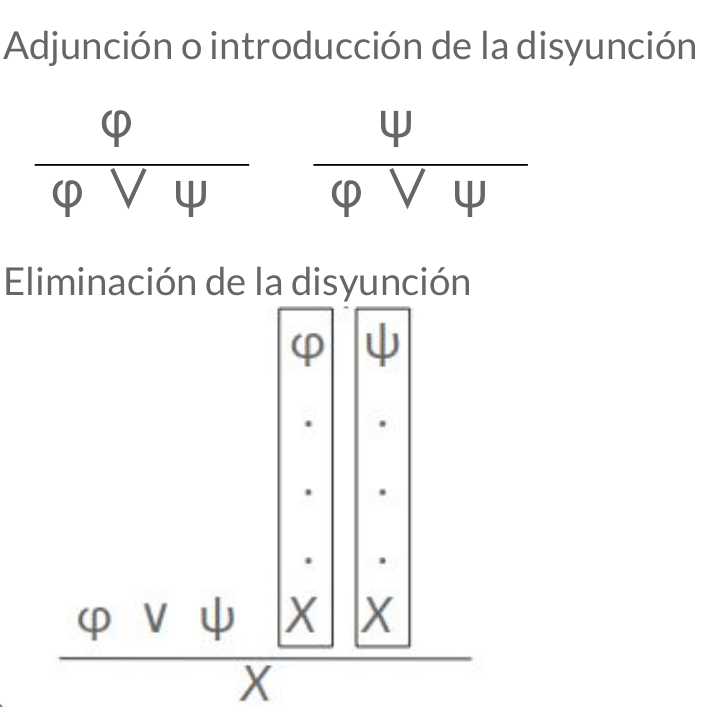
\includegraphics[width=0.5\textwidth]{images/reglas_inferencia.png}

  Utilice las reglas de inferencia anteriores para probar que:
  \begin{enumerate}
    \setcounter{enumi}{4}
    \item $p \vee q \vdash q \vee p$
  \end{enumerate}

\end{frame}


\begin{frame}{Deducción natural: ejemplo 5}
  Utilice las reglas de inferencia anteriores para probar que:
  $$p \vee q \vdash q \vee p$$

  \begin{align*}
    &(1) \quad p \vee q  & \quad (\text{premisa}) \\
    &(2) \quad p  & \quad (\text{supuesto}) \\
    &(3) \quad q \vee p  & \quad (\text{ID2 (2)}) \\
    &(4) \quad q  & \quad (\text{supuesto}) \\
    &(5) \quad q \vee p  & \quad (\text{ID1 (4)}) \\
    \cline{1-2}
    & \quad q \vee p & \quad (\text{ED (1, 2-3, 4-5)})
  \end{align*}

  % Draw the rectangle
  \begin{tikzpicture}[remember picture, overlay]
    \draw[thick] (2.7, 1.87) rectangle (3.7, 2.9);
    \draw[thick] (2.7, 2.97) rectangle (3.7, 4);
  \end{tikzpicture}
\end{frame}


\begin{frame}{Deducción natural: reglas}
  \begin{itemize}
    \item Adjunción o introducción de la negación (IN):
          \begin{equation*}
            \frac{
              \fbox{
                $\begin{array}{c}
                  \upvarphi \\
                  \vdots \\
                  \perp
                \end{array}$
              }
            }{\sim \upvarphi}
          \end{equation*}

    \item Eliminación de la negación (EN):
    $$\dfrac{\Uppsi \quad \sim \Uppsi}{\perp}$$

  \end{itemize}

  Utilice las reglas de inferencia anteriores para probar que:
  \begin{enumerate}
    \setcounter{enumi}{5}
    \item $p \rightarrow \sim p \vdash \sim p$
  \end{enumerate}
\end{frame}


\begin{frame}{Deducción natural: ejemplo 6}
  Utilice las reglas de inferencia anteriores para probar que:
  $$p \rightarrow \sim p \vdash \sim p$$

  \begin{align*}
    &(1) \quad p \rightarrow \sim p  & \quad (\text{premisa}) \\
    &(2) \quad p  & \quad (\text{supuesto}) \\
    &(3) \quad \sim p  & \quad (\text{EI (2, 1)}) \\
    &(4) \quad \perp  & \quad (\text{EN (2-3)}) \\
    \cline{1-2}
    & \qquad \sim p & \quad (\text{IN (2-4)})
  \end{align*}

  % Draw the rectangle
  \begin{tikzpicture}[remember picture, overlay]
    \draw[thick] (2.9, 1.87) rectangle (3.9, 3.5);
  \end{tikzpicture}
\end{frame}


\begin{frame}{Deducción natural: reglas}
  \begin{itemize}
    \item Demostración por contradicción (DPC):
          \begin{equation*}
            \frac{
              \fbox{
                $\begin{array}{c}
                  \sim \upvarphi \\
                  \vdots \\
                  \perp
                \end{array}$
              }
            }{\upvarphi}
          \end{equation*}
  \end{itemize}

  Utilice las reglas de inferencia anteriores para probar que:
  \begin{enumerate}
    \setcounter{enumi}{6}
    \item $\sim p \rightarrow \perp \quad \vdash p$
  \end{enumerate}
\end{frame}


\begin{frame}{Deducción natural: ejemplo 7}
  Utilice las reglas de inferencia anteriores para probar que:
  $$\sim p \rightarrow \perp \quad \vdash p$$

  \begin{align*}
    &(1) \quad \sim p \rightarrow \perp  & \quad (\text{premisa}) \\
    &(2) \quad \sim p  & \quad (\text{supuesto}) \\
    &(3) \quad \perp  & \quad (\text{EI (2, 1)}) \\
    &(4) \quad \sim (\sim p)  & \quad (\text{IN (2-3)}) \\
    \cline{1-2}
    & \qquad p & \quad (\text{EDN (4)})
  \end{align*}

  % Draw the rectangle
  \begin{tikzpicture}[remember picture, overlay]
    \draw[thick] (2.9, 2.5) rectangle (3.9, 3.5);
  \end{tikzpicture}
\end{frame}


\end{document}
